\section{Full-Bank Continuous-Influence Extension}

\label{sec:continuous-extension}

This separately frozen retrospective extension tests Linear, ACVTT, ResUNet, SMamba-UNet and the validated variable-depth ArSSR interface. The earlier closure and historical inference families remain intact. The new eight-model family includes original HAT/SwinIR/SAINT observations without re-inference, retains numerically failed models and uses identical examination bootstrap draws within each cohort. It does not correct for the entire research history.

Acquired inputs, all 417 depth-selected targets per model, masks, Q1/Q99 scale, context grid, four Rademacher seeds, amplitudes, clipping and fixed-count covariates remain unchanged. All new models use the existing .90 gate; HAT/SwinIR retain .85. Response arrays are hash-bound before target access. ArSSR densifies only its two observed anchors using the native deterministic initializer at the actual physical spacing; intermediate planes are not acquired evidence. Its target-only query is checked against the full native normalized-input routine at all nine contexts before outcome evaluation.

\begin{table*}[t]\centering\footnotesize
\caption{Continuous-influence audit of the full 13-model bank. BC: $|\rho_I|-|\rho_{count}|$ for error alignment; FC: exactly-one-anchor partial correlation adjusting span, asymmetry and examination. Intervals use a NEW simultaneous family of eight scheduled models per cohort/endpoint, retaining numerical failures. Min./status is the minimum of three frozen amplitude/sign rank checks; gates are .85 for HAT/SwinIR and .90 otherwise. Interface NA is not a measured null. Linear is an analytical control. All individual checks, legacy intervals and secondary signs are in the supplement/CSV.}
\label{tab:continuous-big}\setlength{\tabcolsep}{3pt}
\begin{tabular}{lrrlrrl}\toprule
& \multicolumn{3}{c}{fastMRI: 24 examinations} & \multicolumn{3}{c}{IXI: 115 examinations}\\
Model & BC [sim. CI] & FC [sim. CI] & Min./status & BC [sim. CI] & FC [sim. CI] & Min./status\\\midrule
Linear & 0.077 [0.061, 0.092] & 0.371 [0.067, 0.675] & 0.982 / PASS & 0.083 [0.077, 0.088] & -0.076 [-0.126, -0.026] & 0.989 / PASS\\
Cubic & NA & NA & NA (interface) & NA & NA & NA (interface)\\
ACVTT & 0.092 [0.078, 0.105] & 0.223 [-0.044, 0.491] & 0.789 / \textbf{FAIL} & 0.082 [0.071, 0.092] & 0.194 [0.129, 0.259] & 0.898 / \textbf{FAIL}\\
Res-SRDiff & NA & NA & NA (interface) & NA & NA & NA (interface)\\
ArSSR & 0.082 [0.069, 0.094] & 0.430 [0.237, 0.622] & 0.964 / PASS & 0.123 [0.118, 0.128] & 0.562 [0.508, 0.617] & 0.999 / PASS\\
CycleINR-style & NA & NA & NA (interface) & NA & NA & NA (interface)\\
ResUNet & 0.094 [0.078, 0.110] & -0.103 [-0.260, 0.054] & 0.989 / PASS & 0.127 [0.120, 0.134] & 0.400 [0.325, 0.475] & 0.998 / PASS\\
Pix2Pix-GAN & NA & NA & NA (interface) & NA & NA & NA (interface)\\
SwinIR & 0.093 [0.078, 0.109] & 0.365 [0.181, 0.549] & 0.942 / PASS & 0.093 [0.081, 0.105] & 0.265 [0.180, 0.350] & 0.880 / PASS\\
SAINT-style & 0.033 [0.012, 0.054] & 0.380 [0.226, 0.534] & 0.951 / PASS & 0.133 [0.124, 0.141] & 0.417 [0.372, 0.463] & 0.996 / PASS\\
I3Net & NA & NA & NA (interface) & NA & NA & NA (interface)\\
HAT & 0.103 [0.085, 0.121] & 0.474 [0.285, 0.663] & 0.964 / PASS & 0.098 [0.088, 0.108] & 0.270 [0.177, 0.362] & 0.930 / PASS\\
SMamba-UNet & 0.078 [0.060, 0.097] & 0.202 [-0.011, 0.415] & 0.918 / PASS & 0.096 [0.083, 0.109] & 0.304 [0.215, 0.393] & 0.968 / PASS\\\bottomrule\end{tabular}\end{table*}

Of 16 measured model/cohort strata, 14 pass numerical stability and 14 also have positive simultaneous beyond-count intervals. The five newly scheduled implementations contribute 10 measured strata and 8 such supported strata. Technical incompatibility, numerical failure and a null association are separately reported.

\begin{figure*}[t]\centering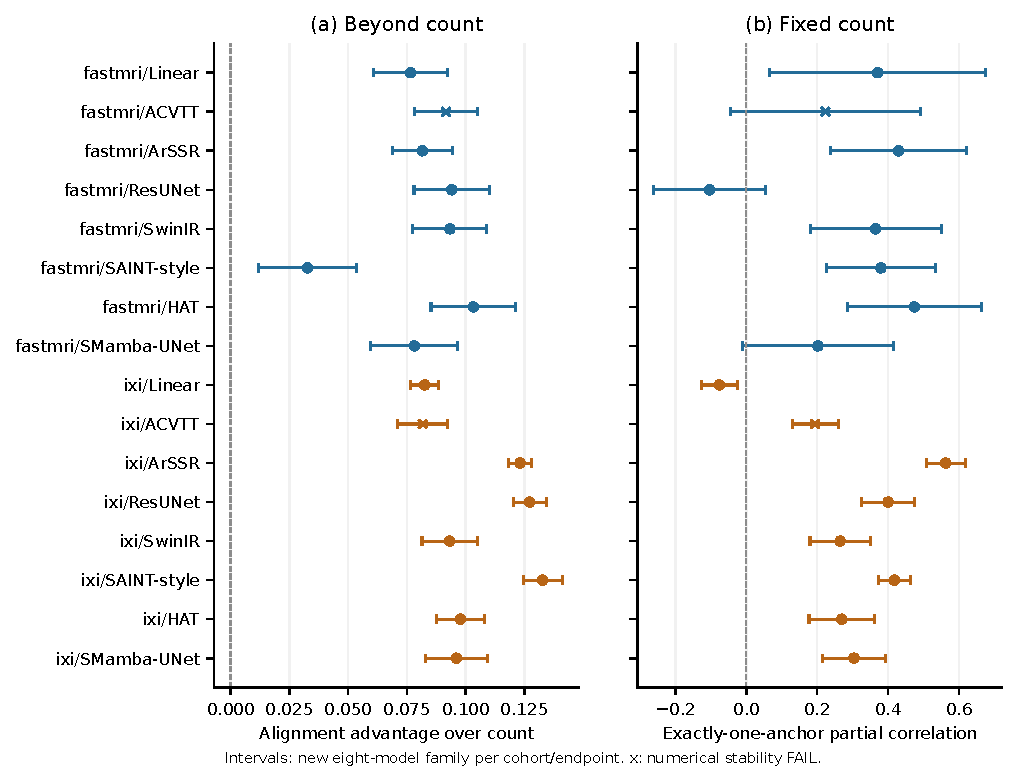
\includegraphics[width=.98\textwidth]{continuous_influence_all_models.pdf}

\caption{Every estimable continuous-influence model/cohort, under the new simultaneous comparison families. Crosses retain numerical failures. This figure is not filtered by favorable results.}\end{figure*}

\begin{table*}[t]\centering\scriptsize

\caption{fastmri: all three rank-stability checks; every model retained. Legacy null/fail results belong to their original information contracts.}

\begin{tabular}{lrrrrll}\toprule Model & $+.005$ & $+.02$ & $-.01$ & Gate & Stability & Beyond-count claim\\\midrule

Linear & 0.981955 & 0.996626 & 0.999749 & 0.90 & PASS & SUPPORTED\\

Cubic & NA & NA & NA & NA & NA & INELIGIBLE\\

ACVTT & 0.789229 & 0.958875 & 0.998067 & 0.90 & FAIL & NUMERICAL FAIL\\

Res-SRDiff & NA & NA & NA & NA & NA & INELIGIBLE\\

ArSSR & 0.994519 & 0.963778 & 0.999756 & 0.90 & PASS & SUPPORTED\\

CycleINR-style & NA & NA & NA & NA & NA & INELIGIBLE\\

ResUNet & 0.989373 & 0.991655 & 0.994260 & 0.90 & PASS & SUPPORTED\\

Pix2Pix-GAN & NA & NA & NA & NA & NA & INELIGIBLE\\

SwinIR & 0.978903 & 0.942054 & 0.977629 & 0.85 & PASS & SUPPORTED\\

SAINT-style & 0.950686 & 0.983707 & 0.996964 & 0.90 & PASS & SUPPORTED\\

I3Net & NA & NA & NA & NA & NA & INELIGIBLE\\

HAT & 0.985533 & 0.964290 & 0.972553 & 0.85 & PASS & SUPPORTED\\

SMamba-UNet & 0.926954 & 0.917539 & 0.993569 & 0.90 & PASS & SUPPORTED\\

\bottomrule\end{tabular}\end{table*}

\begin{table*}[t]\centering\scriptsize

\caption{ixi: all three rank-stability checks; every model retained. Legacy null/fail results belong to their original information contracts.}

\begin{tabular}{lrrrrll}\toprule Model & $+.005$ & $+.02$ & $-.01$ & Gate & Stability & Beyond-count claim\\\midrule

Linear & 0.991735 & 0.989113 & 0.998750 & 0.90 & PASS & SUPPORTED\\

Cubic & NA & NA & NA & NA & NA & INELIGIBLE\\

ACVTT & 0.897623 & 0.968612 & 0.997814 & 0.90 & FAIL & NUMERICAL FAIL\\

Res-SRDiff & NA & NA & NA & NA & NA & INELIGIBLE\\

ArSSR & 0.999716 & 0.998991 & 0.999903 & 0.90 & PASS & SUPPORTED\\

CycleINR-style & NA & NA & NA & NA & NA & INELIGIBLE\\

ResUNet & 0.998505 & 0.997747 & 0.998715 & 0.90 & PASS & SUPPORTED\\

Pix2Pix-GAN & NA & NA & NA & NA & NA & INELIGIBLE\\

SwinIR & 0.880314 & 0.950539 & 0.911329 & 0.85 & PASS & SUPPORTED\\

SAINT-style & 0.996704 & 0.996341 & 0.997466 & 0.90 & PASS & SUPPORTED\\

I3Net & NA & NA & NA & NA & NA & INELIGIBLE\\

HAT & 0.929824 & 0.957558 & 0.934796 & 0.85 & PASS & SUPPORTED\\

SMamba-UNet & 0.992994 & 0.968170 & 0.993162 & 0.90 & PASS & SUPPORTED\\

\bottomrule\end{tabular}\end{table*}

The expanded audit also defines boundaries: acvtt on fastMRI fails the frozen numerical gate (minimum 0.789); acvtt on IXI fails the frozen numerical gate (minimum 0.898); linear on IXI has a negative fixed-count association (-0.076, simultaneous CI [-0.126,-0.026]). Numerical PASS and beyond-count support do not imply a positive fixed-count association.

\subsection{All secondary endpoints and amplitudes}

All values below are descriptive; no secondary endpoint replaces alignment or changes claim eligibility. BC is absolute-correlation advantage over count; FC is exactly-one-anchor partial rank correlation. Undefined values remain NA.

\begin{table*}[t]\centering\scriptsize

\caption{fastmri, alignment: complete descriptive BC/FC by amplitude.}

\begin{tabular}{lrrrr}\toprule Model & $+.01$ (primary) & $+.005$ & $+.02$ & $-.01$\\\midrule

Linear & 0.0766/0.3706 & 0.0793/0.4456 & 0.0754/0.3415 & 0.0765/0.3702\\

ACVTT & 0.0917/0.2234 & 0.0762/-0.1112 & 0.0942/0.3420 & 0.0909/0.2080\\

ArSSR & 0.0816/0.4296 & 0.0866/0.5142 & 0.0625/0.0525 & 0.0819/0.4341\\

ResUNet & 0.0941/-0.1030 & 0.0988/-0.0172 & 0.0921/-0.1134 & 0.0971/-0.0721\\

SwinIR & 0.0933/0.3650 & 0.1011/0.3531 & 0.0730/0.3641 & 0.0956/0.3686\\

SAINT-style & 0.0328/0.3798 & 0.0466/0.3741 & 0.0326/0.3928 & 0.0335/0.3838\\

HAT & 0.1033/0.4741 & 0.1118/0.4954 & 0.0855/0.4393 & 0.1044/0.4837\\

SMamba-UNet & 0.0782/0.2019 & 0.0924/0.2106 & 0.0507/0.1470 & 0.0768/0.2055\\

\bottomrule\end{tabular}\end{table*}

\begin{table*}[t]\centering\scriptsize

\caption{fastmri, observable: complete descriptive BC/FC by amplitude.}

\begin{tabular}{lrrrr}\toprule Model & $+.01$ (primary) & $+.005$ & $+.02$ & $-.01$\\\midrule

Linear & 0.0867/-0.3633 & 0.0895/-0.4396 & 0.0856/-0.3346 & 0.0866/-0.3638\\

ACVTT & 0.0968/-0.1924 & 0.0833/0.1324 & 0.0998/-0.3228 & 0.0961/-0.1785\\

ArSSR & 0.0828/-0.4002 & 0.0868/-0.4881 & 0.0664/-0.0247 & 0.0831/-0.4056\\

ResUNet & 0.0948/0.1007 & 0.0995/0.0126 & 0.0929/0.1117 & 0.0976/0.0711\\

SwinIR & 0.0923/-0.3203 & 0.1020/-0.3245 & 0.0697/-0.3072 & 0.0947/-0.3230\\

SAINT-style & 0.0299/-0.3370 & 0.0450/-0.3330 & 0.0296/-0.3489 & 0.0308/-0.3410\\

HAT & 0.0967/-0.3828 & 0.1066/-0.4131 & 0.0775/-0.3464 & 0.0987/-0.3988\\

SMamba-UNet & 0.0854/-0.1982 & 0.0996/-0.1846 & 0.0593/-0.1746 & 0.0835/-0.1939\\

\bottomrule\end{tabular}\end{table*}

\begin{table*}[t]\centering\scriptsize

\caption{fastmri, disagreement: complete descriptive BC/FC by amplitude.}

\begin{tabular}{lrrrr}\toprule Model & $+.01$ (primary) & $+.005$ & $+.02$ & $-.01$\\\midrule

Linear & 0.0658/-0.2305 & 0.0710/-0.3074 & 0.0648/-0.2145 & 0.0657/-0.2251\\

ACVTT & 0.0717/-0.2738 & 0.0553/0.0508 & 0.0759/-0.3531 & 0.0723/-0.2643\\

ArSSR & 0.0141/-0.1993 & 0.0207/-0.2625 & -0.0012/0.0393 & 0.0141/-0.2049\\

ResUNet & 0.0537/-0.0020 & 0.0597/-0.0623 & 0.0495/0.0208 & 0.0546/-0.0145\\

SwinIR & 0.0192/-0.2573 & 0.0261/-0.2318 & 0.0143/-0.2614 & 0.0264/-0.2659\\

SAINT-style & 0.0029/-0.2386 & 0.0033/-0.2380 & 0.0082/-0.2501 & 0.0044/-0.2447\\

HAT & 0.0419/-0.2135 & 0.0519/-0.2351 & 0.0269/-0.1699 & 0.0365/-0.2245\\

SMamba-UNet & 0.0193/-0.1918 & 0.0298/-0.1879 & 0.0057/-0.1781 & 0.0188/-0.1870\\

\bottomrule\end{tabular}\end{table*}

\begin{table*}[t]\centering\scriptsize

\caption{fastmri, paired error: complete descriptive BC/FC by amplitude.}

\begin{tabular}{lrrrr}\toprule Model & $+.01$ (primary) & $+.005$ & $+.02$ & $-.01$\\\midrule

Linear & 0.0516/0.0018 & 0.0509/0.0251 & 0.0519/-0.0050 & 0.0515/0.0061\\

ACVTT & 0.0489/-0.0232 & 0.0449/-0.1159 & 0.0473/0.0104 & 0.0469/-0.0293\\

ArSSR & 0.0972/0.1503 & 0.0925/0.1571 & 0.1038/0.1374 & 0.0974/0.1475\\

ResUNet & 0.0487/0.0716 & 0.0479/0.1096 & 0.0509/0.0833 & 0.0499/0.0921\\

SwinIR & 0.0798/-0.0255 & 0.0805/0.0220 & 0.0636/-0.0477 & 0.0737/-0.0340\\

SAINT-style & 0.0312/0.0458 & 0.0436/0.0446 & 0.0257/0.0489 & 0.0305/0.0434\\

HAT & 0.0397/-0.0003 & 0.0370/0.0025 & 0.0386/0.0236 & 0.0473/0.0028\\

SMamba-UNet & 0.0600/-0.0629 & 0.0652/-0.0287 & 0.0519/-0.0675 & 0.0596/-0.0561\\

\bottomrule\end{tabular}\end{table*}

\begin{table*}[t]\centering\scriptsize

\caption{fastmri, reference error: complete descriptive BC/FC by amplitude.}

\begin{tabular}{lrrrr}\toprule Model & $+.01$ (primary) & $+.005$ & $+.02$ & $-.01$\\\midrule

Linear & 0.0003/-0.0013 & 0.0008/0.0100 & 0.0005/-0.0065 & 0.0003/0.0030\\

ACVTT & 0.0037/-0.0361 & 0.0068/-0.0953 & 0.0051/-0.0210 & 0.0055/-0.0390\\

ArSSR & 0.0466/0.1325 & 0.0420/0.1313 & 0.0536/0.1430 & 0.0467/0.1298\\

ResUNet & 0.0037/0.1130 & 0.0046/0.1510 & 0.0017/0.1173 & 0.0025/0.1325\\

SwinIR & 0.0386/-0.0075 & 0.0343/0.0350 & 0.0309/-0.0386 & 0.0315/-0.0103\\

SAINT-style & 0.0104/0.0180 & 0.0122/0.0169 & 0.0057/0.0184 & 0.0098/0.0162\\

HAT & 0.0011/-0.0157 & 0.0083/-0.0210 & 0.0053/0.0046 & 0.0055/-0.0202\\

SMamba-UNet & 0.0077/-0.0691 & 0.0027/-0.0622 & 0.0120/-0.0750 & 0.0077/-0.0658\\

\bottomrule\end{tabular}\end{table*}

\begin{table*}[t]\centering\scriptsize

\caption{fastmri, companion error: complete descriptive BC/FC by amplitude.}

\begin{tabular}{lrrrr}\toprule Model & $+.01$ (primary) & $+.005$ & $+.02$ & $-.01$\\\midrule

Linear & 0.0930/0.0177 & 0.0923/0.0464 & 0.0932/0.0105 & 0.0929/0.0220\\

ACVTT & 0.0913/0.0001 & 0.0873/-0.1114 & 0.0895/0.0496 & 0.0893/-0.0115\\

ArSSR & 0.1327/0.1836 & 0.1282/0.1942 & 0.1382/0.1465 & 0.1328/0.1802\\

ResUNet & 0.0934/0.0359 & 0.0928/0.0757 & 0.0952/0.0439 & 0.0946/0.0584\\

SwinIR & 0.1141/-0.0342 & 0.1192/0.0193 & 0.0904/-0.0591 & 0.1096/-0.0405\\

SAINT-style & 0.0471/0.0718 & 0.0682/0.0654 & 0.0410/0.0790 & 0.0459/0.0656\\

HAT & 0.0737/-0.0090 & 0.0753/-0.0014 & 0.0663/0.0215 & 0.0816/-0.0006\\

SMamba-UNet & 0.1056/-0.0354 & 0.1193/0.0160 & 0.0859/-0.0417 & 0.1046/-0.0260\\

\bottomrule\end{tabular}\end{table*}

\begin{table*}[t]\centering\scriptsize

\caption{ixi, alignment: complete descriptive BC/FC by amplitude.}

\begin{tabular}{lrrrr}\toprule Model & $+.01$ (primary) & $+.005$ & $+.02$ & $-.01$\\\midrule

Linear & 0.0826/-0.0757 & 0.0825/-0.0848 & 0.0838/-0.0732 & 0.0827/-0.0740\\

ACVTT & 0.0817/0.1941 & 0.1126/0.4152 & 0.0928/0.2304 & 0.0825/0.1945\\

ArSSR & 0.1232/0.5624 & 0.1232/0.5620 & 0.1233/0.5652 & 0.1232/0.5623\\

ResUNet & 0.1272/0.4001 & 0.1281/0.4182 & 0.1259/0.3740 & 0.1273/0.4028\\

SwinIR & 0.0933/0.2649 & 0.0608/0.1787 & 0.1091/0.3466 & 0.0924/0.2684\\

SAINT-style & 0.1328/0.4174 & 0.1331/0.4151 & 0.1320/0.4224 & 0.1327/0.4154\\

HAT & 0.0978/0.2695 & 0.0836/0.2359 & 0.1082/0.3325 & 0.1001/0.2818\\

SMamba-UNet & 0.0961/0.3038 & 0.0935/0.2900 & 0.0989/0.2825 & 0.0965/0.3148\\

\bottomrule\end{tabular}\end{table*}

\begin{table*}[t]\centering\scriptsize

\caption{ixi, observable: complete descriptive BC/FC by amplitude.}

\begin{tabular}{lrrrr}\toprule Model & $+.01$ (primary) & $+.005$ & $+.02$ & $-.01$\\\midrule

Linear & 0.1104/-0.0070 & 0.1093/0.0171 & 0.1099/-0.0090 & 0.1104/-0.0065\\

ACVTT & 0.0925/-0.2245 & 0.1215/-0.4200 & 0.1050/-0.2677 & 0.0932/-0.2249\\

ArSSR & 0.1377/-0.5038 & 0.1376/-0.5014 & 0.1379/-0.5078 & 0.1377/-0.5034\\

ResUNet & 0.1337/-0.3584 & 0.1349/-0.3828 & 0.1325/-0.3312 & 0.1336/-0.3581\\

SwinIR & 0.1035/-0.2531 & 0.0687/-0.1666 & 0.1201/-0.3173 & 0.1020/-0.2573\\

SAINT-style & 0.1417/-0.3589 & 0.1430/-0.3659 & 0.1402/-0.3575 & 0.1417/-0.3584\\

HAT & 0.1094/-0.2895 & 0.0949/-0.2626 & 0.1202/-0.3439 & 0.1120/-0.3025\\

SMamba-UNet & 0.1089/-0.3818 & 0.1057/-0.3611 & 0.1125/-0.3575 & 0.1091/-0.3929\\

\bottomrule\end{tabular}\end{table*}

\begin{table*}[t]\centering\scriptsize

\caption{ixi, disagreement: complete descriptive BC/FC by amplitude.}

\begin{tabular}{lrrrr}\toprule Model & $+.01$ (primary) & $+.005$ & $+.02$ & $-.01$\\\midrule

Linear & 0.0189/0.0025 & 0.0193/0.0085 & 0.0249/-0.0107 & 0.0191/0.0003\\

ACVTT & 0.0329/-0.2916 & 0.0468/-0.5019 & 0.0342/-0.3259 & 0.0334/-0.2869\\

ArSSR & 0.0405/-0.4122 & 0.0403/-0.4100 & 0.0411/-0.4128 & 0.0403/-0.4108\\

ResUNet & 0.0562/-0.3783 & 0.0568/-0.4014 & 0.0544/-0.3499 & 0.0566/-0.3809\\

SwinIR & 0.0474/-0.3890 & 0.0344/-0.3195 & 0.0484/-0.4290 & 0.0475/-0.3931\\

SAINT-style & 0.0341/-0.1687 & 0.0327/-0.1787 & 0.0344/-0.1684 & 0.0340/-0.1697\\

HAT & 0.0518/-0.2868 & 0.0460/-0.2092 & 0.0554/-0.3651 & 0.0511/-0.2943\\

SMamba-UNet & 0.0674/-0.4701 & 0.0702/-0.4766 & 0.0535/-0.3861 & 0.0692/-0.4777\\

\bottomrule\end{tabular}\end{table*}

\begin{table*}[t]\centering\scriptsize

\caption{ixi, paired error: complete descriptive BC/FC by amplitude.}

\begin{tabular}{lrrrr}\toprule Model & $+.01$ (primary) & $+.005$ & $+.02$ & $-.01$\\\midrule

Linear & 0.0542/0.0359 & 0.0534/0.0256 & 0.0478/0.0207 & 0.0540/0.0335\\

ACVTT & 0.0200/-0.1320 & 0.0198/-0.2128 & 0.0253/-0.1417 & 0.0198/-0.1263\\

ArSSR & 0.0393/-0.0712 & 0.0395/-0.0706 & 0.0388/-0.0679 & 0.0394/-0.0710\\

ResUNet & 0.0273/-0.1928 & 0.0271/-0.2005 & 0.0288/-0.1776 & 0.0269/-0.1970\\

SwinIR & 0.0099/-0.2154 & 0.0036/-0.2201 & 0.0167/-0.2266 & 0.0100/-0.1930\\

SAINT-style & 0.0377/0.0368 & 0.0398/0.0391 & 0.0362/0.0301 & 0.0377/0.0363\\

HAT & 0.0094/-0.0639 & 0.0071/-0.0053 & 0.0109/-0.1038 & 0.0116/-0.0567\\

SMamba-UNet & -0.0125/-0.1672 & -0.0163/-0.1833 & 0.0019/-0.1194 & -0.0144/-0.1724\\

\bottomrule\end{tabular}\end{table*}

\begin{table*}[t]\centering\scriptsize

\caption{ixi, reference error: complete descriptive BC/FC by amplitude.}

\begin{tabular}{lrrrr}\toprule Model & $+.01$ (primary) & $+.005$ & $+.02$ & $-.01$\\\midrule

Linear & 0.0081/0.0266 & 0.0075/0.0207 & 0.0017/0.0159 & 0.0079/0.0241\\

ACVTT & 0.0115/-0.1105 & 0.0194/-0.2031 & 0.0093/-0.1258 & 0.0118/-0.1060\\

ArSSR & 0.0035/-0.0547 & 0.0032/-0.0539 & 0.0040/-0.0527 & 0.0033/-0.0543\\

ResUNet & 0.0167/-0.1124 & 0.0170/-0.1194 & 0.0154/-0.1050 & 0.0171/-0.1151\\

SwinIR & 0.0274/-0.2263 & 0.0249/-0.2191 & 0.0235/-0.2248 & 0.0258/-0.2027\\

SAINT-style & 0.0015/0.0285 & 0.0034/0.0251 & 0.0005/0.0228 & 0.0015/0.0272\\

HAT & 0.0286/-0.0576 & 0.0276/-0.0157 & 0.0289/-0.0972 & 0.0273/-0.0567\\

SMamba-UNet & 0.0501/-0.2342 & 0.0537/-0.2419 & 0.0354/-0.1805 & 0.0519/-0.2370\\

\bottomrule\end{tabular}\end{table*}

\begin{table*}[t]\centering\scriptsize

\caption{ixi, companion error: complete descriptive BC/FC by amplitude.}

\begin{tabular}{lrrrr}\toprule Model & $+.01$ (primary) & $+.005$ & $+.02$ & $-.01$\\\midrule

Linear & 0.0860/0.0556 & 0.0850/0.0399 & 0.0798/0.0341 & 0.0858/0.0532\\

ACVTT & 0.0432/-0.1390 & 0.0495/-0.1972 & 0.0505/-0.1469 & 0.0431/-0.1325\\

ArSSR & 0.0688/-0.0756 & 0.0690/-0.0752 & 0.0685/-0.0719 & 0.0690/-0.0755\\

ResUNet & 0.0569/-0.2096 & 0.0569/-0.2157 & 0.0583/-0.1919 & 0.0565/-0.2143\\

SwinIR & 0.0386/-0.1869 & 0.0263/-0.2025 & 0.0472/-0.1973 & 0.0370/-0.1780\\

SAINT-style & 0.0642/0.0488 & 0.0665/0.0544 & 0.0626/0.0435 & 0.0643/0.0495\\

HAT & 0.0388/-0.0556 & 0.0339/0.0034 & 0.0412/-0.0878 & 0.0413/-0.0482\\

SMamba-UNet & 0.0175/-0.0850 & 0.0136/-0.1105 & 0.0311/-0.0423 & 0.0157/-0.0899\\

\bottomrule\end{tabular}\end{table*}

\paragraph{Batch execution correction.}
ACVTT/IXI and ResUNet/both cohorts initially failed the pre-response batch1-versus-batch4 equality check, although their single-sample adapters matched the native single-sample predictor exactly. Before any target evaluation for those three units, an engineering addendum fixed both nominal and perturbed predictions to single-sample execution. The original $10^{-5}$ native-output and $10^{-6}$ repeat tolerances were unchanged; all nine contexts were rechecked. The original failures are retained. Completed units keep their validated batch path, including the ACVTT/fastMRI numerical-stability failure. No scientific outcome determined this repair's scope; thresholds, cohorts and perturbations were unchanged.

\subsection{Limits and provenance}

Linear is not a neural replication. Adapted implementations and the ArSSR/CycleINR code lineage limit independence of architectural counts. Fixed-count associations can retain geometry and clipping effects. The cohort is reused retrospectively; simultaneous intervals quantify sampling variation within these fixed analyses, not historical selection. No new covariance or calibrated reliability claim follows automatically. All earlier negative findings and NEEDS HUMAN CONFIRMATION data/ethics items remain valid.

\paragraph{Reproduction.} The protocol, frozen hashes, raw responses, independent physical-anchor embedding checks, all 26 bank rows, bootstrap replicates and execution logs are retained in \path{CONTINUOUS_INFLUENCE_EXPANSION/}. Earlier masks, predictions and protocols remain read-only.